\documentclass[letterpaper, 12pt]{article}
\usepackage[a4paper, total={6in, 10in}]{geometry}
\usepackage{graphicx}
\graphicspath{ {./images/} }
\usepackage{wrapfig}
\usepackage{float}
\usepackage{lipsum}
\floatstyle{boxed}

\title{Applications of The NEAT Algorithm in Deterministic Game Environments}
\date{\today}
\author{John Kechagias\\ Department of Informatics, University Of Piraeus}
\begin{document}

\maketitle

\centerline{\textbf{THIS IS A WORK IN PROGRESS}}

\begin{abstract}
This paper explores the usages of the NEAT algorithm in combination with self-play in
deterministic game environments. The objective is to investigate the speed at which
models can be trained to adopt particular strategies with minimal reliance on training
data and expert knowledge. To achieve this, we develop a game akin to checkers and use
it as a platform to train models to follow specific strategies.
\end{abstract}

\section*{Introduction}

Neuroevolution of augmented topologies (NEAT) \cite{stanley:ec02} is an evolutionary 
algorithm designed to create neural networks. Developed by Kenneth O. Stanley and Risto
Miikkulainen in 2002, NEAT sought to overcome the limitations of fixed-topology neural
networks by allowing evolving networks to adapt their structure as they optimize
for performance.

\section*{Implementation Overview}

An Python implementation of the NEAT algorithm was developed for this paper. The
implementation is based on the original paper \cite{stanley:ec02} with some additions.
The core algorithm remains unchanged, we start by creating a population of genomes,
divide them into species, select a representative for each species, assign fitness
scores to each genome, filter out stagnant species, and generate a the new population
based on the old one. For our purposes, we opted for feedfoward neural networks. Thus,
all mutations have been designed as to retain the feedforward nature of the networks.

\subsection*{Fitness Function}

Self-play was utilized to evaluate the genomes. The intention is to pit the genomes
against the best of the previous generation and calculate their fitness based on the
game results. For the first run, because there is no older generation, we pick five
genomes at random to act as the opponents. Each genome fights a set amount of times
against each opponent in order to get an average score. After all games are completed,
we take the average of the game scores and assign it as the genome's fitness. The
function that outputs a score based on a game record, not only takes into account the
game's result, but also the moves that the model made.

\section*{Game Rules}
The game is played on a five by five board with hexadecimal tiles (see Fig 1). There are
two players, denoted as \textbf{red} and \textbf{blue}. Players start on opposite
corners of the board with one piece each. Each board tile can hold a maximum of ten
pieces. We say that a player owns a tile when he has pieces on it. The blue player moves
first and then play alternates between sides. The goal of the game is to eliminate all
of the opponent's pieces. There are two moves available to each player, \textbf{transfer}
and \textbf{production}.

\subsection*{Transfer Move}
Players can select any number of their owned pieces from a tile and transfer them to a 
neighbouring tile. For this move to be valid, the following conditions must be met:
\begin{itemize}
  \item The starting tile and the destination tile are adjacent.
  \item The number of selected pieces must not exceed the total number of pieces on the
    starting tile.
  \item The total number of pieces on the destination tile must not exceed the maximum 
    allowed number of pieces on a tile.
\end{itemize}
If the destination tile is occupied by the opposing player, a fight ensues. During the
fight, the number of tiles possessed by the player with the greater quantity is 
subtracted from both sides. For example, blue player transfers six troops from tile
\((4, 0)\) to \((3, 1)\):


\begin{figure}[H]
  \begin{minipage}[c]{.5\textwidth}
    \centering
    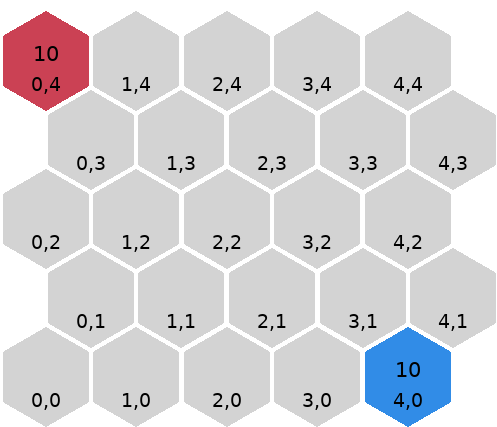
\includegraphics[width=0.9\textwidth]{transfer_example_1.png}
    \caption{Before the Transfer Move.}
  \end{minipage}%
  \begin{minipage}[c]{.5\textwidth} \centering
    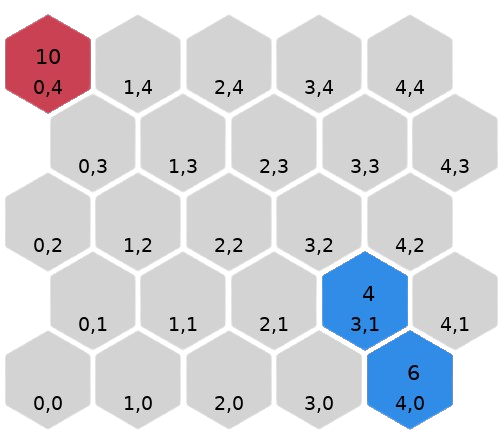
\includegraphics[width=0.9\textwidth]{transfer_example_2.png}
    \caption{After the Transfer Move.}
  \end{minipage}
\end{figure}

\subsection*{Production Move}

Players can select a tile they occupy and add one more piece to it. For this move to be
valid, the number of pieces on the tile must be less than the maximum allowed number of
pieces on a tile. For example, blue player produces a piece on tile \((3, 1)\):

\begin{figure}[H]
  \begin{minipage}[c]{.5\textwidth}
    \centering
    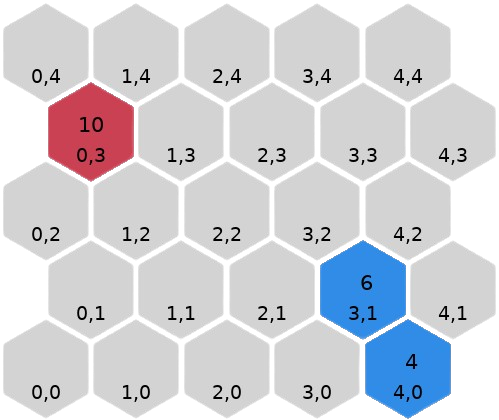
\includegraphics[width=0.9\textwidth]{production_example_1.png}
    \caption{Before the Production Move.}
  \end{minipage}%
  \begin{minipage}[c]{.5\textwidth} \centering
    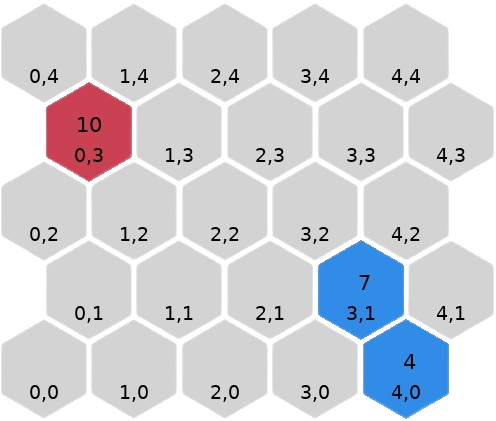
\includegraphics[width=0.9\textwidth]{production_example_2.png}
    \caption{After the Production Move.}
  \end{minipage}
\end{figure}

\section*{Methodology}

\subsection*{Input Preparation}

The following protocol was adopted for evolving strategies in the aforementioned game.
The game board is interpreted as a five by five matrix, with each cell representing a
tile on the board. The value in each cell shows the number of soldiers present on that
tile. To differentiate between players' pieces, blue pieces are represented with
positive numbers and red pieces with negative numbers.

\subsection*{Move Searching} 

The idea is to search throught all the possible moves and countermoves up to a given
depth and utilize the neural network for assessing each game state. The job of the
neural networks is to take the matrix form of a game state as input and output a score
indicating how favorable the position is for the player whose pieces are represented
with positive numbers. Since the networks are designed to evaluate positions only from
the perspective of the player with positive pieces, when we want to evaluate a position
from the perspective of the other player (whose pieces are represented with negative
numbers), we must multiply the matrix by \(-1\) to switch perspectives. We employ the
principal variation search to examine all possible moves up to a given depth. For
evaluating each game state we utilize the neural network. Whenever we change player
turns, we adjust the matrix by multiplying it by \(-1\) before feeding it to the model
to switch perspectives. Once the search is complete, we select the move that results in
the most advantageous game state for the current player.

\bibliographystyle{plain}
\bibliography{refs}
\end{document}
